%
% File acl2019.tex
%
%% Based on the style files for ACL 2018, NAACL 2018/19, which were
%% Based on the style files for ACL-2015, with some improvements
%%  taken from the NAACL-2016 style
%% Based on the style files for ACL-2014, which were, in turn,
%% based on ACL-2013, ACL-2012, ACL-2011, ACL-2010, ACL-IJCNLP-2009,
%% EACL-2009, IJCNLP-2008...
%% Based on the style files for EACL 2006 by 
%%e.agirre@ehu.es or Sergi.Balari@uab.es
%% and that of ACL 08 by Joakim Nivre and Noah Smith

\documentclass[11pt,a4paper]{article}
\usepackage[hyperref]{acl2019}
\usepackage{times}
\usepackage{latexsym}

\usepackage{url}
\usepackage{graphicx}
\graphicspath{ {./image/} }
\hbadness=10000
%\aclfinalcopy % Uncomment this line for the final submission
%\def\aclpaperid{***} %  Enter the acl Paper ID here

%\setlength\titlebox{5cm}
% You can expand the titlebox if you need extra space
% to show all the authors. Please do not make the titlebox
% smaller than 5cm (the original size); we will check this
% in the camera-ready version and ask you to change it back.

\newcommand\BibTeX{B\textsc{ib}\TeX}

\title{Instructions for ACL 2019 Proceedings}

\author{First Author \\
  Affiliation / Address line 1 \\
  Affiliation / Address line 2 \\
  Affiliation / Address line 3 \\
  \texttt{email@domain} \\\And
  Second Author \\
  Affiliation / Address line 1 \\
  Affiliation / Address line 2 \\
  Affiliation / Address line 3 \\
  \texttt{email@domain} \\}

\date{}

\begin{document}
\maketitle
\begin{abstract}
  % Automatic summarization research has made substantial progress thanks to novel methods and datasets. Manual evaluation approaches so far either ignore content and focus on fluency, or require expert annotators but nevertheless suffer from low inter-annotator agreement due to the complexity of the task. In the few cases where the contents of the summary are evaluated, the evaluation is biased due to using a single reference summary, which results in different summaries of equal quality being rated according to their similarity to the reference. In this paper, we propose a Highlight-bAsed Evaluation of Single document Summarization (HArnESS). Our proposal assesses summaries against the original document, facilitated through manually highlighted salient content which can be reused in future studies. Furthermore it does not require expert annotators, avoids reference bias and provides absolute instead of ranked evaluation of systems.
  Automatic summarization research has made substantial progress thanks to novel methods and datasets. 
  %OLD:
  %However, a well-accepted manual evaluation for content such as Pyramid requires expert annotation which is often not available for many datasets. As such, current practices choose to assess the content by directly comparing the summary against the original document or a reference summary. 
  %Our finding found that these practices are not suitable for long document or dataset that only provides a single reference summary per document as these cases are often result in scores that have high variability between judges' assessment due to bias. 
  %AV: I would replace the 3 sentences above with something like: 
  Despite this progress, most manual evaluation focuses on fluency but not on the content of the summaries. Those that do, typically use a single reference summary for comparison, either directly or through questions, which introduces a bias towards a single correct answer for a task where this assumption doesn't hold.
  To address this issue, we propose Highlight-bAsed Evaluation of Single document Summarization (HArnESS) that provides assessment of a summary against the original document, facilitated through manually highlighted salient content. The highlights lower the variability of the judges' assessment and are reusable in future studies. Furthermore it does not require expert annotators, avoids reference bias and provides absolute instead of ranked evaluation of the systems.
  
\end{abstract}

\section{Introduction}
Research in automatic summarization has made headway over the years with single document summarization as the front-runner due to the availability of large datasets  \citep{Sandhaus2008, Hermann2015, Shashi2018} and novel methods \citep{See2017, Kryscinski2018, Shashi2018}. Despite this progress, there is a large number of studies (e.g., See2017) that didn't perform any manual evaluation at all. Those that do, typically did not take account of bias that comes from comparing to a single reference summary, either directly \citep{Celikyilmaz2018, Tan2017} or through questions \citep{Shashi2018, Narayan2018}; or have little agreements on how to evaluate content of the summaries. As the rest of them that don't, they were mostly relying on automatic evaluation such as ROUGE \citep{Lin2004}, but it has been shown in \citet{Louis2013} that for single document summarization case ROUGE is inaccurate due to reference bias.

Up to now, too little attention has been paid to build a consensus in manual evaluation framework which has eventually lead to a fragmented field and many unnecessary system evaluation rerun due to non-reusable results. Summarization field used to have a common manual evaluation practice that is established through DUC such as Pyramid method \citep{Nenkova2004} but then the method would need expert annotators for every new dataset which is costly. Furthermore, the method is also prone to reference bias when there is only one summary available for every document.


In this paper we propose Highlight-bAsed Evaluation of Single document Summarization (HArnESS) which makes three contributions: (1) We present a new way to assess a content of summary by comparing it against the original document, facilitated through manually highlighted salient document. (2) We provide a complete manual evaluation framework for evaluating the quality of summary that yields reusable result and does not require expert annotators. (3) We provide a new augmented annotation for XSum dataset.  

\section{Data}
For our experiment, we use the extreme summarization (XSum) Dataset \citep{Shashi2018} which comprises of BBC article and summary pairs. The summary in the XSum dataset has a big proportion of novel unigrams compared to other more popular dataset such as CNN/Daily Mail or NY Times. This makes the dataset suitable for our experiment since we don't want the judges to be biased towards extractive methods which makes the process of assessment easier compared to the abstractive methods. In other words, we expect in an abstractive setting, the task of reading an article will be more laborous and prone to disagreement between judges.

We didn't use the whole test set portion for evaluation, but only sampled 50 articles from it for the annotation and evaluation purpose following the human evaluation practice from the \citet{Shashi2018}'s author.

For the peer summaries, we use the Topic-aware Convolutional Sequence to Sequence (T-CONVS2s) model \footnote{\url{https://github.com/EdinburghNLP/XSum}} \citep{Shashi2018} and Pointer-Generator Networks model \footnote{\url{https://github.com/abisee/pointer-generator}} \citep{See2017} as the comparisons. We obtained both summary result by directly running the code on our sampled dataset. 

\section{Highlight Annotation}
The highlight annotation is a manual process where we ask human to read the XSum article and then highlight words or phrases that are considered as important for the article. To perform the task, we use the Amazon HIT (Human Intelligence Task). Each of the 50 articles is annotated ten times done separately. 

We gave the Turkers a guidance on how to do the highlight task using the 5W1H (Who, What, When, Where, Why and How) principles \citep{Robertson1946} that is a common practice in journalism. Since the dataset is a news article, the most important information would be part of the articles that answer the 5W1H question. However, we don't expect every single annotation to cover all the answer to the 5W1H, instead we want the annotation to have a more diverse highlights which cover different viewpoints of the article which is why we limited each annotator to a maximum of 30 words highlight.

At the end of the task, we performed a sanity checking to ensure the reliability of the annotation result by asking the Turker to answer a True/False question about part of the article. We expect each Turker that had performed the highlight would be able to answer the question correctly since they had read the whole article. We rejected all annotations that failed to correctly answer the sanity question. Table \ref{table:highlightedwords} shows three out of ten annotation for one article \footnote{\url{https://www.bbc.co.uk/newsround/17546358}}. 

\begin{table}[!h]
  \small
  \begin{tabular}{lp{6.5cm}}
  No. & Highlighted Words \\
  \hline
  1 & {[}'Mr Bezos', 'found the engines from the Apollo 11 space rocket', '4,300 metres below the surface of the Atlantic Ocean', 'going to ask Nasa', 'display', 'engines', 'Museum of Flight'{]} \\
  2 & {[}'engines broke off from the spaceship after blast off', 'crashed somewhere in the Atlantic Ocean .', 'Mr Bezos', 'found the engines from the Apollo 11'{]}                                          \\
  3 & {['engines from the Apollo 11 space rocket - the craft that carried the first men to the moon in 1969 .', 'Mr Bezos', 'Atlantic Ocean', 'Apollo 11 unfold on television']} \\
  \end{tabular}
\caption{Three samples of highlight annotation for article ID 17546358 }
\label{table:highlightedwords}
\end{table}
   

\section{Evaluation}
We evaluated two models: TConvs2s \citep{Shashi2018} and PTGen \citep{See2017} using the following evaluation frameworks. For the evaluation, we use the direct assessment approach instead of relative ranking as this would enable us to reuse the results for subsequent evaluation with different models furthermore we isolate each model summary assessment in its own task thereby avoiding a bias from having seen different models. In addition to that, we also use a 1-100 rating scale instead of 1-5 rating scale that is normally used for summarization approach. For each model's summary, we ask three different Turkers to judge the quality.

\subsection{Content Evaluation}
In content evaluation, we run two different settings: the assessment by comparing the summary against the reference summary and against the article directly. 

\paragraph{Comparison against the reference summary} The head-to-head comparison of model and reference summary is a norm in DUC \footnote{Document Understanding Conference \url{http://duc.nist.gov/
use}} and automatic assessment such as ROUGE and BLEU. For this task we ask the Turker to assess a randomly model summary against the reference summary of the same article using the recall and precision metrics.

The recall and precision are represented by these two statements:\textit{`All important information is present in the summary'} and \textit{`Only important information is in the summary.'} The first statement denotes how good is the article coverage of the summary, while the second one denotes how precise is the information conveyed by the summary. The benefit of having an analogous metric to the automatic assessment would means that we are able to calculate the $F_1$ score from the recall and precision just like the automatic score. We also measure the variability of the scores by calculating the coefficient of variation ($cv$). The $cv$ score is the ratio between the sample standard deviation and sample mean as the following equation.
\begin{equation}
  c_v = \frac{\sigma}{\bar{x}}
\end{equation}
where $\sigma$ is the standard deviation, and $\bar{x}$ is the mean. Since, our samples are quite small, we need to use the unbiased version as the following equation.
\begin{equation}
  \hat{c_v} = (1 + \frac{1}{4n})c_v
\end{equation}

Using the coefficient of variation we can compare the variability of different models.

Table \ref{table:refsummresult} shows the evaluation result for PTGEN and TCONVS2S models.

\begin{table}[]
  \small
  \begin{tabular}{llll}
  \hline
  \multicolumn{4}{l}{PTGEN}                                          \\
  \hline
            & precision        & recall           & f1               \\
  mean      & 44.24            & 38.34            & 35.83        \\
  std       & 27.08        & 28.20        & 25.57        \\
  $\hat{cv}$        & 0.78         & 0.84         & 0.82         \\
  \hline
  \multicolumn{4}{l}{TCONVS2S}                                       \\
  \hline
  & precision & recall           & f1                                 \\
  mean      & 46.75 & 36.45 & 36.83 \\
  std       & 25.86        & 27.91        & 25.19        \\
  $\hat{cv}$        & 0.78         & 0.90         & 0.85        
  \end{tabular}
\caption{The mean, standard deviation and coefficient of variability for PTGEN and TCONVS2S models using comparison against reference summary.}
\label{table:refsummresult}
\end{table}

\paragraph{Comparison against the article} For the task, we gave the Turker one summary (could be model or reference summary) and the related article. There are however, two different configurations: facilitated with highlight guidance (guided) and without any facilitation (unguided). The highlight guidance is intended to help the Turker to decide the summary content quality when making the judgment. We use the same rating scale of 1-100 and the same metrics: precision and recall. Table \ref{table:articlesummresult} shows the evaluation result for Reference, PTGEN and TCONVS2S models.

\begin{table}[]
  \small
  \begin{tabular}{p{0.5cm}p{0.6cm}p{0.6cm}p{0.6cm}|p{0.6cm}p{0.6cm}p{0.6cm}}
    \hline
  \multicolumn{4}{l}{Guided Reference} & \multicolumn{3}{l}{Unguided Reference} \\
  \hline
        & Prec  & Rec  & F1    & Prec  & Rec  & F1         \\
  mean  & 67.90      & 56.83   & 55.25 & 66.01         & 52.45      & 50.67     \\
  std   & 25.36      & 26.26   & 25.43 & 26.36         & 29.18      & 25.28     \\
  $\hat{cv}$    & 0.49       & 0.63    & 0.61  & 0.48          & 0.67       & 0.61      \\
  \hline
  \multicolumn{4}{l}{Guided PTGEN}     & \multicolumn{3}{l}{Unguided PTGEN}     \\
  \hline
        & Prec  & Rec  & F1     & Prec  & Rec  & F1         \\
  mean  & 50.94      & 44.41   & 42.17 & 48.57         & 39.21      & 37.80     \\
  std   & 27.54      & 30.68   & 26.28 & 27.31         & 30.11      & 26.84     \\
  $\hat{cv}$    & 0.73       & 0.86    & 0.81  & 0.73          & 0.90       & 0.84      \\
  \hline
  \multicolumn{4}{l}{Guided TCONVS2S}  & \multicolumn{3}{l}{Unguided TCONVS2S}  \\
  \hline
        & Prec  & Rec  & F1     & Prec  & Rec  & F1            \\
  mean  & 57.42      & 49.95   & 47.00 & 52.55         & 41.04      & 39.25     \\
  std   & 29.63      & 31.23   & 26.91 & 27.45         & 26.18      & 24.38     \\
  $\hat{cv}$    & 0.67       & 0.80    & 0.71  & 0.75          & 0.83       & 0.81     
  \end{tabular}
  \caption{The mean, standard deviation and coefficient of variability for Guided and unguided Reference, PTGEN and TCONVS2S models using comparison against article.}
\label{table:articlesummresult}
  \end{table}

\subsection{Sentence Quality Evaluation}
In sentence quality evaluation, we ask the Turker to rate the sentence summary alone on two metrics: sentence clarity and fluency. For clarity, the Turker is asked whether the summary is easy to be understood of which there should be no difficulties in identifying the referents of the noun phrases (every noun/place/event should be well-specified) or understanding the meaning of the sentence. While for fluency, the Turker is asked whether the summary sounds natural and has no grammar-related problem that makes the text difficult to read.
 
\section{Discussion}
In this section, we are going to discuss several insights gained from the annotation and evaluation processes.

\subsection{Annotation Agreement}
The average inter-annotator's agreement for 50 articles measured using Fleiss Kappa \citep{Josep1971} is 0.185. Table \ref{image:interannotator} shows the inter-annotator agreement for 50 articles. This result shows only a slight agreement for each article, however, we considered it as normal since one article may have different viewpoints, for example in Table \ref{table:highlightedwords} there are three different viewpoints on one article.

\begin{figure}[h!]
  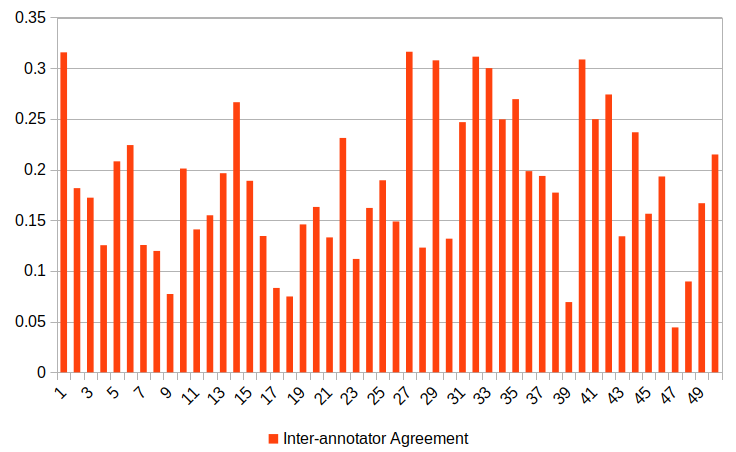
\includegraphics[width=8cm]{annotator}
  \caption{The inter-annotator agreement of highlight annotation for 50 articles}
  \label{image:interannotator}
\end{figure}

\subsection{Variability Analysis}
The coefficient of variability results show a slight improvement for the guided models compares to the unguided ones which means that the judges are more agreeing with each other over the perceived quality of a summary. For the PTGEN model, the guided $F_1$ score is 0.03 lower than the unguided while the for the TCONVS2S model, the guided $F_1$ score is 0.1 lower than the unguided. Meanwhile there is no difference between the guided and unguided. To understand the cause, we look into several examples to see why this has happened. 

The first example is the article ID 36328049\footnote{\url{https://www.bbc.co.uk/news/world-africa-36328049}}. Table \ref{table:result36328049} and Table \ref{table:example36328049} shows the result and summary text for the models and reference.

\begin{table}[h!]
  \small
  \begin{tabular}{p{1cm}p{1cm}p{1cm}p{1cm}p{1cm}}
    \hline
  \multicolumn{5}{l}{TCONVS2S} \\
  \hline                                
  F1 Guided & F1 Unguided & Guided-Unguided & cv Guided & cv Unguided \\
  1.98      & 64.56       & -62.58   & 0         & 0.44        \\
  \hline
  \multicolumn{5}{l}{PTGEN}    \\
  \hline                                
  F1 Guided & F1 Unguided & Guided-Unguided & cv Guided & cv Unguided \\
  67.61     & 41.32       & 26.29    & 0.37      & 1.05       
\end{tabular}
\caption{The result from PTGEN, TCONVS2S, and Reference for Article ID 36328049.}
\label{table:result36328049}
\end{table}

\begin{table}[h!]
  \small
  \begin{tabular}{lp{5cm}}
  Model     & Summary Text   \\
  \hline
  PTGEN     & “a nigerian refugee has been rescued from a number of pupils after being kidnapped by islamic state ( is ) militants in northern nigeria .”   \\
  TCONVS2S  & “nigerian schoolgirl who was abducted by boko haram militants in nigeria has been reunited with her parents .”                                        \\
  REFERENCE & “the first of the missing nigerian schoolgirls to be rescued since her capture two years ago has had an emotional reunion with her mother .”         
  \end{tabular}
  \caption{The summaries text from PTGEN, TCONVS2S, and Reference for Article ID 36328049.}
  \label{table:example36328049}
\end{table}

For both models, the cv of the unguided is higher than the guided ones. We checked closely into the highlights and the articles (see Appendix), and we found that the cause of the high variance is because without the guidance, judges are more to disagree the salient contents since the article is long and has several viewpoints. But with proper guidance, judges are more consistent in giving a rating.

Another example is article ID 38204334\footnote{\url{http://www.bbc.co.uk/news/uk-38204334}}. In this article, the TCONVS2s successfully shows the most important part of the article which are also highlighted which is why the judges are more consistent in giving a high rating. 

\begin{table}[h!]
  \small
  \begin{tabular}{lp{5cm}}
  Model     & Summary Text   \\
  \hline
  PTGEN     & “storm desmond battered parts of the uk and lancashire last winter , according to new figures from the office for national statistics ( ceh )”   \\
  TCONVS2S  & “parts of the uk have been battered by flooding in the past year , according to a new report .”                                        \\
  REFERENCE & “flooding across parts of the uk last winter was the most extreme on record , experts have said .”         
  \end{tabular}
  \caption{The summaries text from PTGEN, TCONVS2S, and Reference for Article ID 38204334.}
  \label{table:example38204334}
\end{table}

\begin{table}[h!]
  \small
  \begin{tabular}{p{1cm}p{1cm}p{1cm}p{1cm}p{1cm}}
    \hline
  \multicolumn{5}{l}{TCONVS2S} \\
  \hline                                
  F1 Guided & F1 Unguided & Guided-Unguided & cv Guided & cv Unguided \\
  86.76      & 37.89       & 48.87   & 0.20         & 0.34        \\
  \hline
  \multicolumn{5}{l}{PTGEN}    \\
  \hline                                
  F1 Guided & F1 Unguided & Guided-Unguided & cv Guided & cv Unguided \\
  41.18     & 62.02       & -20.84    & 0.67      & 0.70       
\end{tabular}
\caption{The result from PTGEN, TCONVS2S, and Reference for Article ID 38204334.}
\label{table:result38204334}
\end{table}

\section{Related Works}
Based on ranking scheme there are three approaches: rating scale \citep{Likert1932} used by \citet{Kryscinski2018}, paired comparison \citep{Thurstone1994} used by \citet{Fan2018, Celikyilmaz2018}; and best-worst scaling \citep{Woodworth1991} used by \citet{Shashi2018}. Then based on subject of comparison, there are head-to-head comparison between system and reference summary \citep{Celikyilmaz2018} and ground truth comparison using the document directly \citep{Shashi2018, Kryscinski2018}. Finally there are also different method in evaluating, for example question-answering method \citep{Clarke2010, Shashi2018}. In addition to that, several researches \citep{Nallapati2016a, See2017, Gehrmann2018} did not employ manual evaluation but instead opted to do qualitative analysis directly on the system summary.

\section*{Acknowledgments}

The acknowledgments should go immediately before the references.  Do
not number the acknowledgments section. Do not include this section
when submitting your paper for review. \\

\noindent \textbf{Preparing References:} \\
Include your own bib file like this:
\verb|\bibliographystyle{acl_natbib}|
\verb|\bibliography{acl2019}| 

where \verb|acl2019| corresponds to a acl2019.bib file.
\bibliography{acl2019}
\bibliographystyle{acl_natbib}

\appendix

\section{Appendices}
\label{sec:appendix}
Appendices are material that can be read, and include lemmas, formulas, proofs, and tables that are not critical to the reading and understanding of the paper. 
Appendices should be \textbf{uploaded as supplementary material} when submitting the paper for review. Upon acceptance, the appendices come after the references, as shown here. Use
\verb|\appendix| before any appendix section to switch the section
numbering over to letters.


\section{Supplemental Material}
\label{sec:supplemental}
Submissions may include non-readable supplementary material used in the work and described in the paper. Any accompanying software and/or data should include licenses and documentation of research review as appropriate. Supplementary material may report preprocessing decisions, model parameters, and other details necessary for the replication of the experiments reported in the paper. Seemingly small preprocessing decisions can sometimes make a large difference in performance, so it is crucial to record such decisions to precisely characterize state-of-the-art methods. 

Nonetheless, supplementary material should be supplementary (rather
than central) to the paper. \textbf{Submissions that misuse the supplementary 
material may be rejected without review.}
Supplementary material may include explanations or details of proofs or derivations that do not fit into the paper, lists of features or feature templates, sample inputs and outputs for a system,
pseudo-code or source code, and data. (Source code and data should
be separate uploads, rather than part of the paper).

The paper should not rely on the supplementary material: while the paper
may refer to and cite the supplementary material and the supplementary material will be available to the
reviewers, they will not be asked to review the
supplementary material.


\end{document}
